\section[AB-SFC]{\textbf{Ensaio 3:} Dimensão real e financeira do mercado imobiliário}

\begin{frame}{Nova Narrativa}
\framesubtitle{Participação na execução hipotecária a partir da avaliação de risco}


\begin{figure}
    \centering
    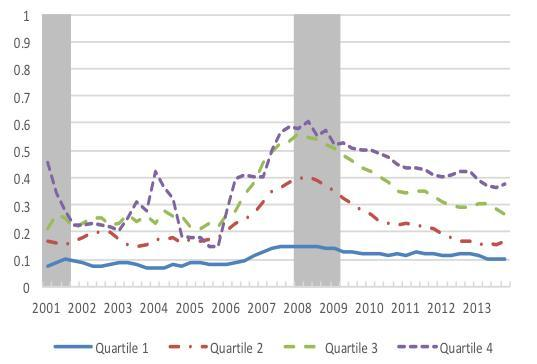
\includegraphics[width=.8\paperwidth, height=.6\paperheight]{figs/NovaNarrativa.png}
\end{figure}

\end{frame}

\begin{frame}{Literatura e suas Lacunas}
\framesubtitle{Integração do lado real e financeiro}

\begin{description}
    \item[SFC:] Lado real $\Leftrightarrow$ financeiro.
    
    \begin{itemize}
        \item Modelo agregado $\nRightarrow$ Fragilidade Financeira
    \end{itemize}
    
    \item[ABM:] Agentes com comportamentos heterogêneos $\Rightarrow$ Emergência de fenômenos macroeconômicos
        \begin{itemize}
        \item Fragilidade Financeira $\nRightarrow$ nem sempre SFC
    \end{itemize}
    
    \item[AB-ABM:] ABM + SFC $\Rightarrow$ Firmas! Firmas! Firmas!
        \begin{itemize}
        \item \textbf{Exceção:} \textcite{carvalho_income_2014}
    \end{itemize}
    
\end{description}
    
\begin{alert}{Lacunas em comum}

Pouca ênfase às famílias e ao investimento residencial

Restrição de crédito (quase sempre) relacionado às firmas

Não investigam as implicações da inflação de ativos

\end{alert}
    
\end{frame}


\begin{frame}{Objetivo e Metodologia}
    
\begin{description}
    \item[Objetivo:]  avaliar as implicações macroeconômicas de um sistema bancário ativo com ciclo de crédito endógeno
\item[Hipótese:] somente as famílias com melhor avaliação de risco investem em imóveis e ampliam a demanda por crédito na medida que seu colateral com os bancos se valoriza $\sim$ Nova Narrativa
    \item[Metodologia:] modelo AB-SFC de simulação com famílias heterogêneas e investimento residencial explicitamente modelado
\end{description}
\end{frame}

\begin{frame}{Estrutura do modelo}

\begin{figure}
    \centering
    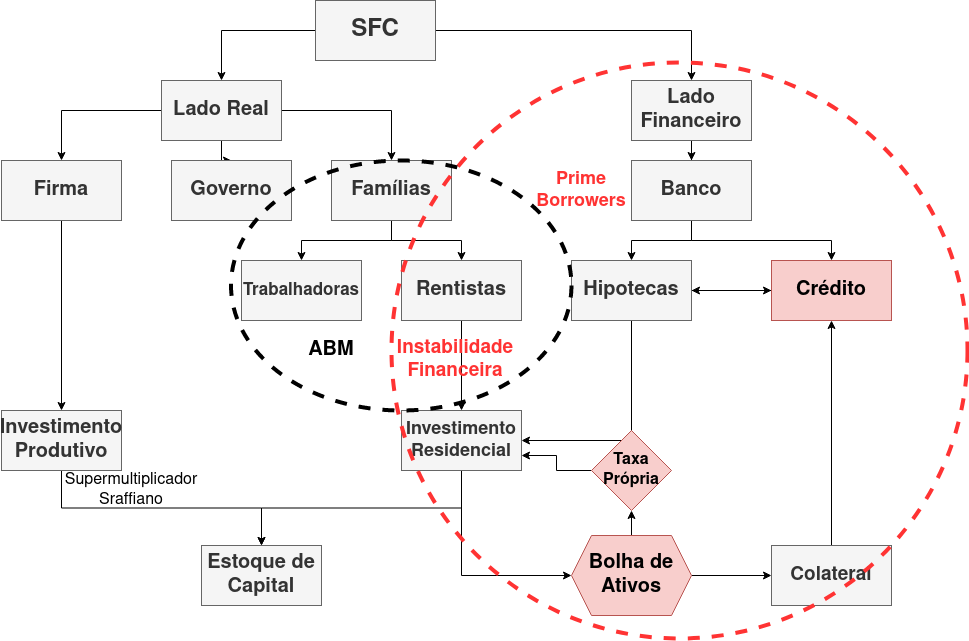
\includegraphics[width=.8\paperwidth, height=.67\paperheight]{./figs/Diagrama_ABSFC.png}
\end{figure}
    
\end{frame}